We will now turn our attention to pruning methods. First we will analyze the functionality of the provided \emph{pruning\_example} function.
We will conclude with a discussion of more general pruning.



\lstset{language=matlab}

\begin{lstlisting}
function pruning_example(x,y)
    
% x: noSamples x 45 (as returned by loaddata)
% y: noSamples x 1 (as returned by loaddata)

tree = classregtree(x,y,'method','classification','categorical',1:45,'minparent',1,'prune','off');
view(tree);
[cost,s,nodes,bestLevel] = test(tree,'cross',x,y);
[cost2,s2,nodes2,bestLevel2] = test(tree,'resubstitution');

prunedTree = prune(tree,'level',bestLevel);
prunedTree2 = prune(tree,'level',bestLevel2);

[mincost,minloc] = min(cost);
[mincost2,minloc2] = min(cost2);


plot(nodes,cost,'b-x','MarkerSize',8)
hold on
plot(nodes(bestLevel+1),cost(bestLevel+1),'ks');
xlabel('Tree size (number of terminal nodes)')
ylabel('Cost')
grid on

plot(nodes2,cost2,'r-x','MarkerSize',8)
plot(nodes2(bestLevel2+1),cost2(bestLevel2+1),'ks');
\end{lstlisting}

The function takes in the examples matrix x, as well as the label matrix y.
These are then passed in to the \emph{classregtree} function
which creates a classification tree that predicts the labels using the columns of the examples matrix.
The parameter 'categorical' tells the function to treat the columns of x (the attributes) as unordered categorical variables
such that each attribute takes on one of a discrete, limited and fixed set of values (here '1' or '0').\\
The parameter 'minparent = 1' dictates that impure nodes that contain 1 or more examples should be split.\\
Since a node that contains 1 example is by definition pure,
this really means that impure nodes that contain 2 or more examples should be split.
The parameters 'prune = off' dictates that there should be no pruning of the tree.\\

This function is actually different than the way we build trees because our model consists of six trees that each classify a given
example.
We extract a label from these six classifications from the trees, with various methods described in the ambiguity section.
The classregtree works differently as it builds one tree, where the leaf nodes are not binary but instead can take one any of the 6 emotion values. For the purpose of this discussion, pruning, this will not matter as it can be applied to each of our trees to yield better classification rates.



\begin{comment}

\begin{figure}[t!]
   \begin{minipage}[b]{0.60\linewidth}
       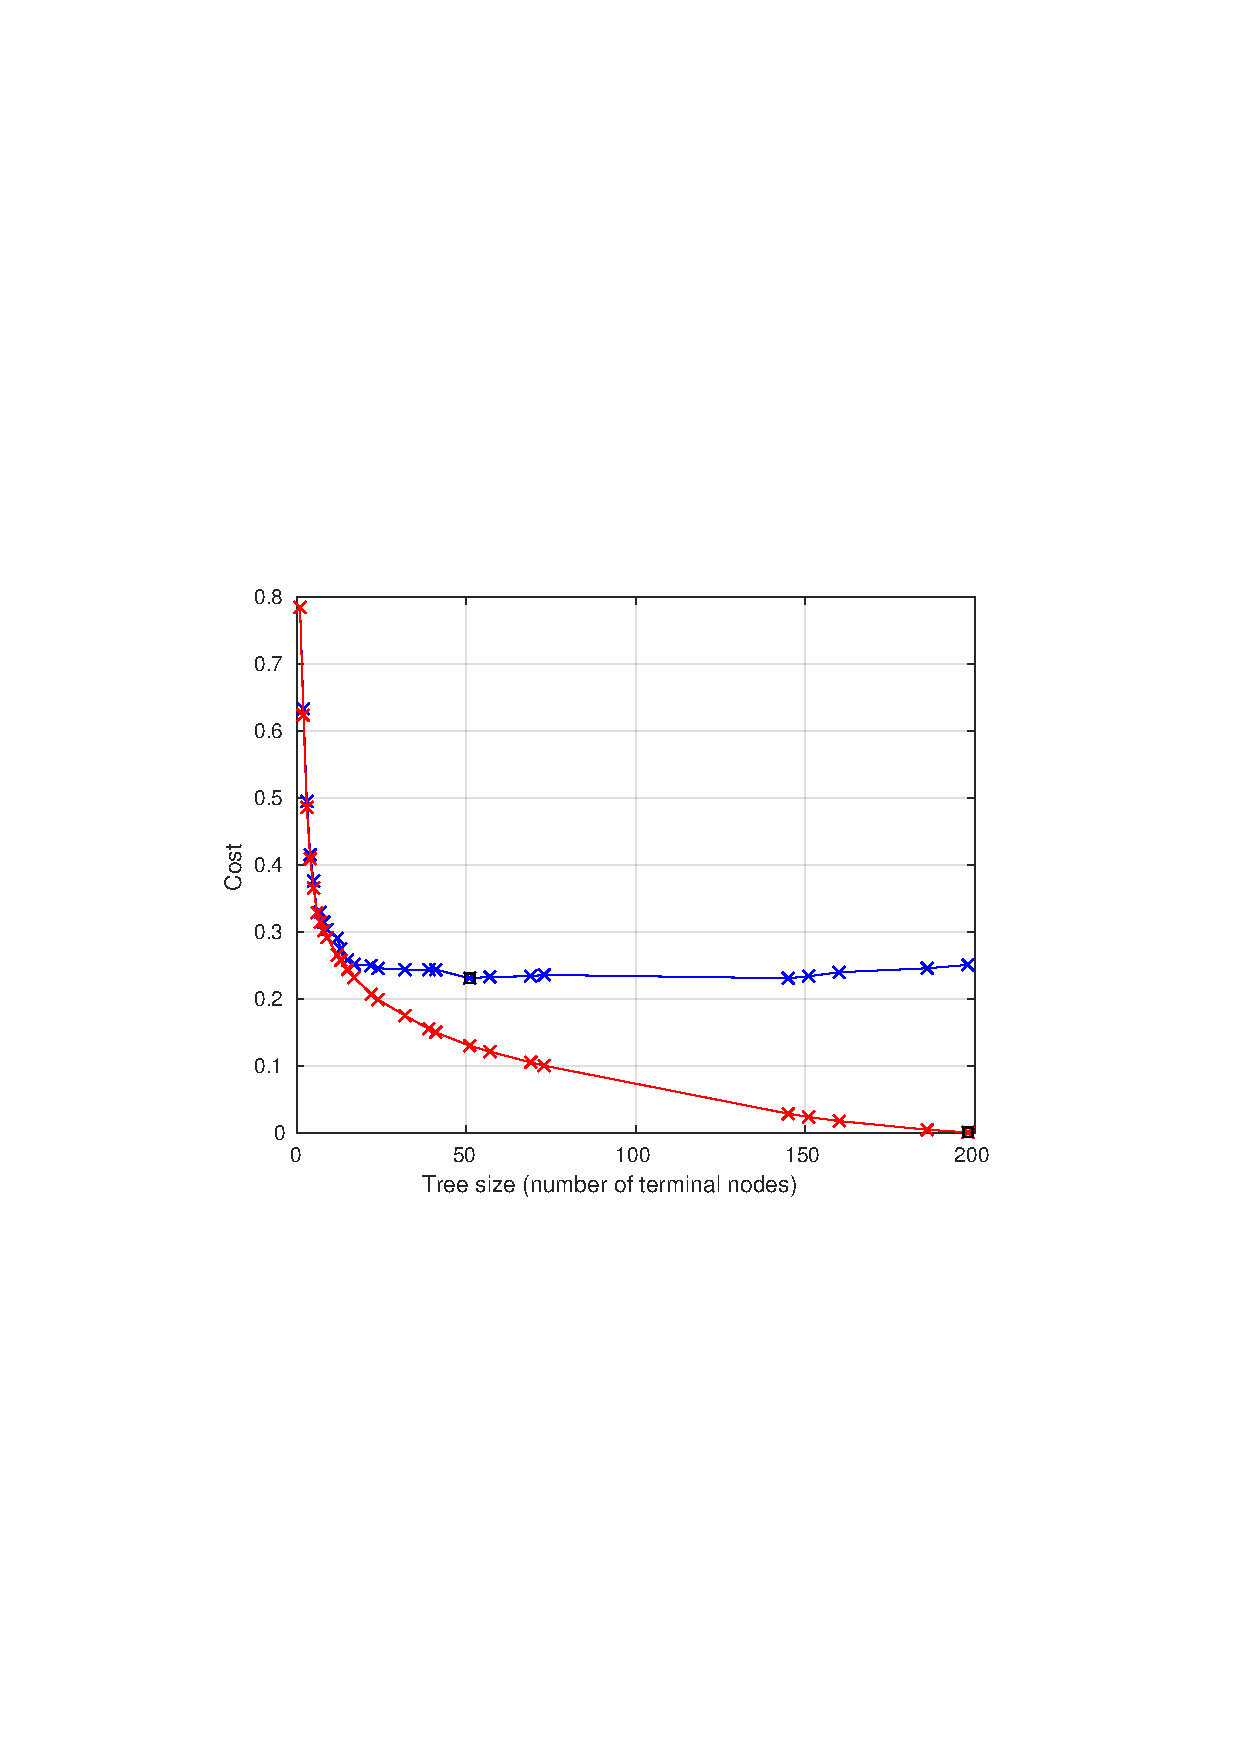
\includegraphics[scale=0.20]{graphs/clean_dataset/clean_pruning.pdf}
      \caption{Légende 1}
   \end{minipage}\hfill

   \begin{minipage}[b]{0.60\linewidth}   
      \centering 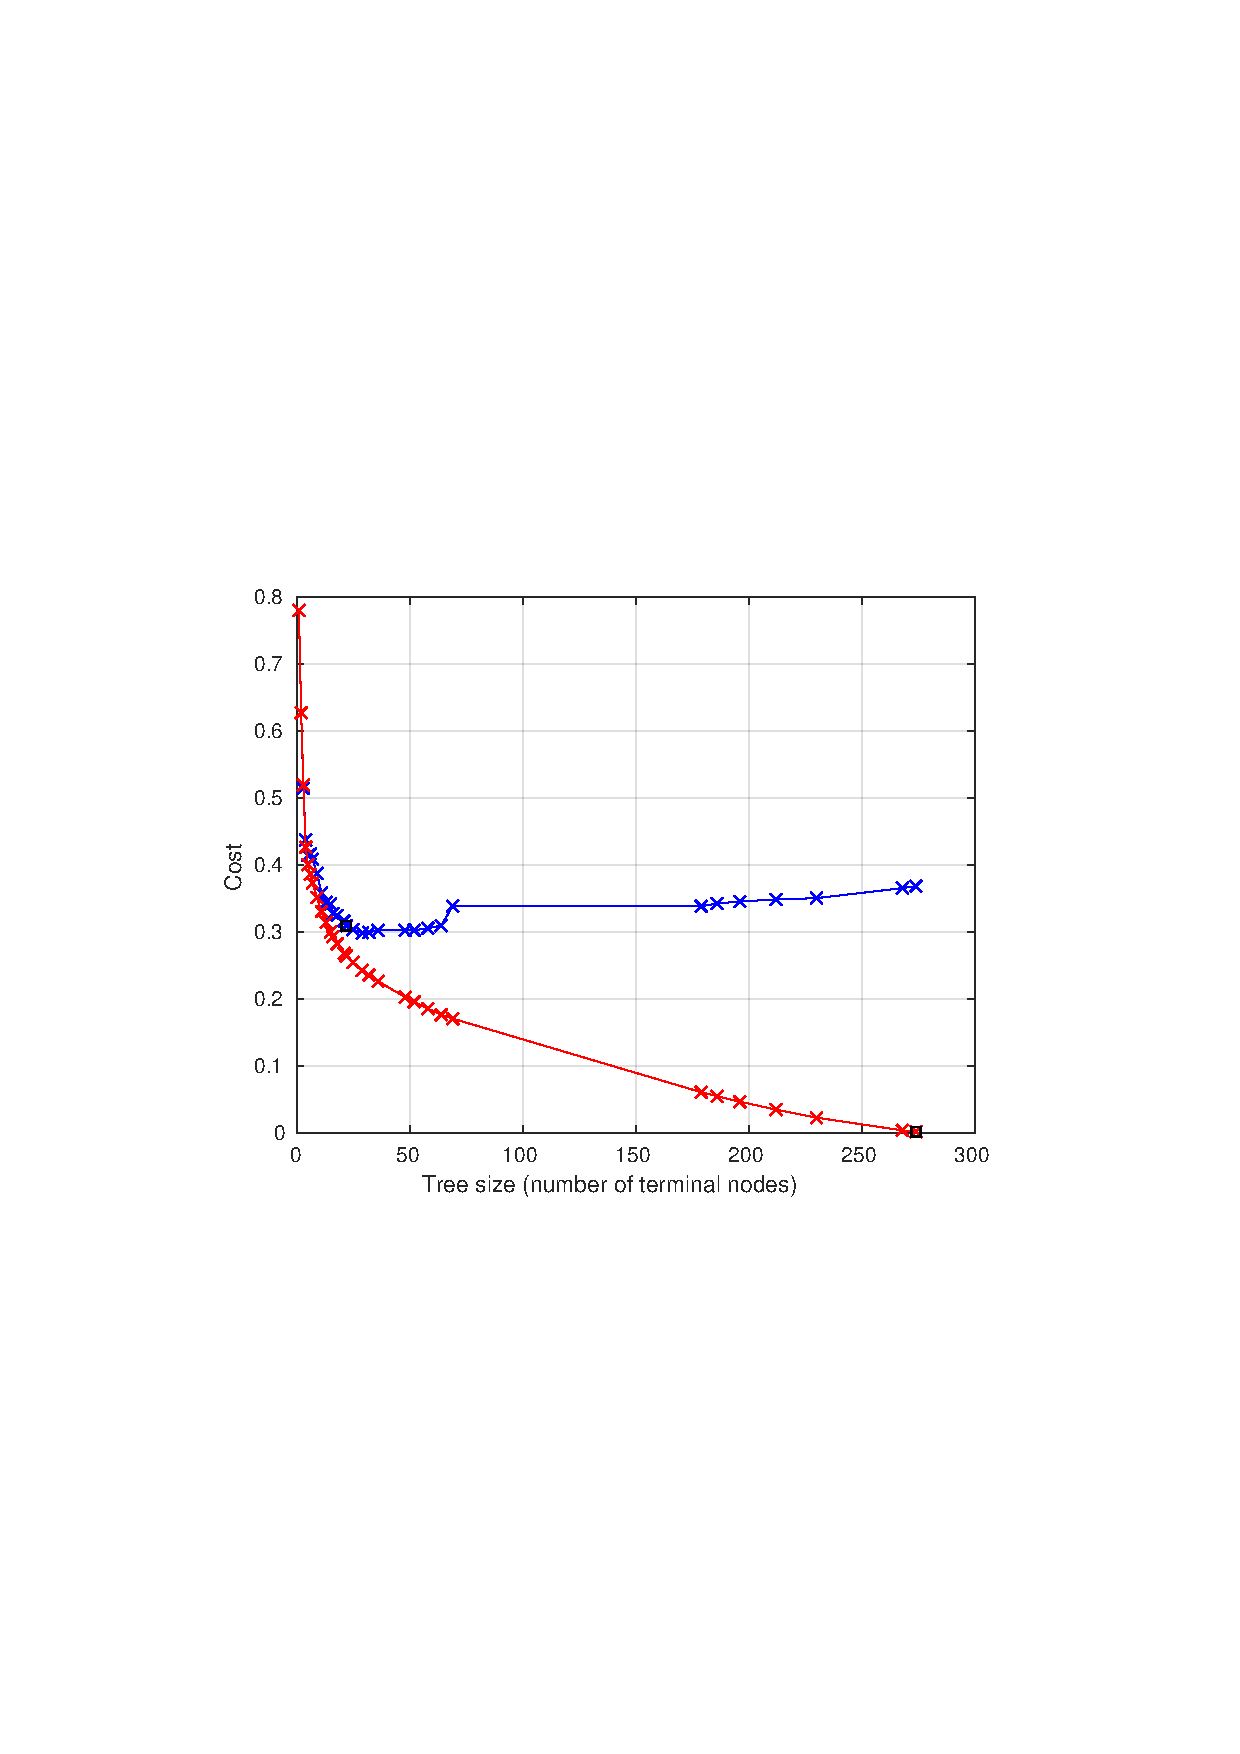
\includegraphics[scale=0.20]{graphs/noisy_dataset/noisy_pruning.pdf}
      \caption{Légende 2}
   \end{minipage}

 \label{fig:cleanprunning2}
\end{figure}


\end{comment}


